\documentclass[twoside]{book}

% Packages required by doxygen
\usepackage{fixltx2e}
\usepackage{calc}
\usepackage{doxygen}
\usepackage[export]{adjustbox} % also loads graphicx
\usepackage{graphicx}
\usepackage[utf8]{inputenc}
\usepackage{makeidx}
\usepackage{multicol}
\usepackage{multirow}
\PassOptionsToPackage{warn}{textcomp}
\usepackage{textcomp}
\usepackage[nointegrals]{wasysym}
\usepackage[table]{xcolor}

% Font selection
\usepackage[T1]{fontenc}
\usepackage[scaled=.90]{helvet}
\usepackage{courier}
\usepackage{amssymb}
\usepackage{sectsty}
\renewcommand{\familydefault}{\sfdefault}
\allsectionsfont{%
  \fontseries{bc}\selectfont%
  \color{darkgray}%
}
\renewcommand{\DoxyLabelFont}{%
  \fontseries{bc}\selectfont%
  \color{darkgray}%
}
\newcommand{\+}{\discretionary{\mbox{\scriptsize$\hookleftarrow$}}{}{}}

% Page & text layout
\usepackage{geometry}
\geometry{%
  a4paper,%
  top=2.5cm,%
  bottom=2.5cm,%
  left=2.5cm,%
  right=2.5cm%
}
\tolerance=750
\hfuzz=15pt
\hbadness=750
\setlength{\emergencystretch}{15pt}
\setlength{\parindent}{0cm}
\setlength{\parskip}{3ex plus 2ex minus 2ex}
\makeatletter
\renewcommand{\paragraph}{%
  \@startsection{paragraph}{4}{0ex}{-1.0ex}{1.0ex}{%
    \normalfont\normalsize\bfseries\SS@parafont%
  }%
}
\renewcommand{\subparagraph}{%
  \@startsection{subparagraph}{5}{0ex}{-1.0ex}{1.0ex}{%
    \normalfont\normalsize\bfseries\SS@subparafont%
  }%
}
\makeatother

% Headers & footers
\usepackage{fancyhdr}
\pagestyle{fancyplain}
\fancyhead[LE]{\fancyplain{}{\bfseries\thepage}}
\fancyhead[CE]{\fancyplain{}{}}
\fancyhead[RE]{\fancyplain{}{\bfseries\leftmark}}
\fancyhead[LO]{\fancyplain{}{\bfseries\rightmark}}
\fancyhead[CO]{\fancyplain{}{}}
\fancyhead[RO]{\fancyplain{}{\bfseries\thepage}}
\fancyfoot[LE]{\fancyplain{}{}}
\fancyfoot[CE]{\fancyplain{}{}}
\fancyfoot[RE]{\fancyplain{}{\bfseries\scriptsize Generated by Doxygen }}
\fancyfoot[LO]{\fancyplain{}{\bfseries\scriptsize Generated by Doxygen }}
\fancyfoot[CO]{\fancyplain{}{}}
\fancyfoot[RO]{\fancyplain{}{}}
\renewcommand{\footrulewidth}{0.4pt}
\renewcommand{\chaptermark}[1]{%
  \markboth{#1}{}%
}
\renewcommand{\sectionmark}[1]{%
  \markright{\thesection\ #1}%
}

% Indices & bibliography
\usepackage{natbib}
\usepackage[titles]{tocloft}
\setcounter{tocdepth}{3}
\setcounter{secnumdepth}{5}
\makeindex

% Hyperlinks (required, but should be loaded last)
\usepackage{ifpdf}
\ifpdf
  \usepackage[pdftex,pagebackref=true]{hyperref}
\else
  \usepackage[ps2pdf,pagebackref=true]{hyperref}
\fi
\hypersetup{%
  colorlinks=true,%
  linkcolor=blue,%
  citecolor=blue,%
  unicode%
}

% Custom commands
\newcommand{\clearemptydoublepage}{%
  \newpage{\pagestyle{empty}\cleardoublepage}%
}

\usepackage{caption}
\captionsetup{labelsep=space,justification=centering,font={bf},singlelinecheck=off,skip=4pt,position=top}

%===== C O N T E N T S =====

\begin{document}

% Titlepage & ToC
\hypersetup{pageanchor=false,
             bookmarksnumbered=true,
             pdfencoding=unicode
            }
\pagenumbering{roman}
\begin{titlepage}
\vspace*{7cm}
\begin{center}%
{\Large Mc\+EA -\/ Multiobjective cellular Evolutionary Algorithm }\\
\vspace*{1cm}
{\large Generated by Doxygen 1.8.11}\\
\end{center}
\end{titlepage}
\clearemptydoublepage
\tableofcontents
\clearemptydoublepage
\pagenumbering{arabic}
\hypersetup{pageanchor=true}

%--- Begin generated contents ---
\chapter{File Index}
\section{File List}
Here is a list of all documented files with brief descriptions\+:\begin{DoxyCompactList}
\item\contentsline{section}{\hyperlink{dtlz_8cu}{dtlz.\+cu} }{\pageref{dtlz_8cu}}{}
\item\contentsline{section}{{\bfseries error.\+h} }{\pageref{error_8h}}{}
\item\contentsline{section}{\hyperlink{mcea_8cu}{mcea.\+cu} }{\pageref{mcea_8cu}}{}
\item\contentsline{section}{\hyperlink{util_8cu}{util.\+cu} }{\pageref{util_8cu}}{}
\item\contentsline{section}{{\bfseries util.\+h} }{\pageref{util_8h}}{}
\end{DoxyCompactList}

\chapter{File Documentation}
\hypertarget{dtlz_8cu}{}\section{dtlz.\+cu File Reference}
\label{dtlz_8cu}\index{dtlz.\+cu@{dtlz.\+cu}}
{\ttfamily \#include \char`\"{}math\+\_\+constants.\+h\char`\"{}}\\*
Include dependency graph for dtlz.\+cu\+:\nopagebreak
\begin{figure}[H]
\begin{center}
\leavevmode
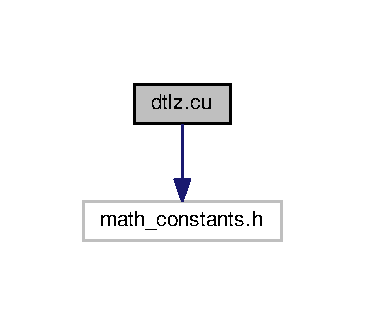
\includegraphics[width=175pt]{dtlz_8cu__incl}
\end{center}
\end{figure}
\subsection*{Functions}
\begin{DoxyCompactItemize}
\item 
\+\_\+\+\_\+device\+\_\+\+\_\+ void \hyperlink{dtlz_8cu_af665aa59f6d550787a3da256e11ca075}{test\+Obj\+Sum} (float $\ast$params, float $\ast$objectives, int param\+\_\+size, int obj\+\_\+size)
\item 
\+\_\+\+\_\+device\+\_\+\+\_\+ void \hyperlink{dtlz_8cu_acb7db8f8aa7dde56b645cf50934148e4}{dtlz1} (float $\ast$params, float $\ast$objectives, int param\+\_\+size, int obj\+\_\+size)
\begin{DoxyCompactList}\small\item\em Function of the D\+T\+L\+Z1 multicriterial optimization problem. \end{DoxyCompactList}\end{DoxyCompactItemize}


\subsection{Detailed Description}
This module contains all used D\+T\+LZ functions. Definition of the functions can be found in\+: Deb, Kalyanmoy, et al. \char`\"{}\+Scalable multi-\/objective optimization test problems.\char`\"{} Evolutionary Computation, 2002. C\+EC\textquotesingle{}02. Proceedings of the 2002 Congress on. Vol. 1. I\+E\+EE, 2002. 

\subsection{Function Documentation}
\index{dtlz.\+cu@{dtlz.\+cu}!dtlz1@{dtlz1}}
\index{dtlz1@{dtlz1}!dtlz.\+cu@{dtlz.\+cu}}
\subsubsection[{\texorpdfstring{dtlz1(float $\ast$params, float $\ast$objectives, int param\+\_\+size, int obj\+\_\+size)}{dtlz1(float *params, float *objectives, int param_size, int obj_size)}}]{\setlength{\rightskip}{0pt plus 5cm}\+\_\+\+\_\+device\+\_\+\+\_\+ void dtlz1 (
\begin{DoxyParamCaption}
\item[{float $\ast$}]{params, }
\item[{float $\ast$}]{objectives, }
\item[{int}]{param\+\_\+size, }
\item[{int}]{obj\+\_\+size}
\end{DoxyParamCaption}
)}\hypertarget{dtlz_8cu_acb7db8f8aa7dde56b645cf50934148e4}{}\label{dtlz_8cu_acb7db8f8aa7dde56b645cf50934148e4}


Function of the D\+T\+L\+Z1 multicriterial optimization problem. 

Calculates the objectives for the D\+T\+L\+Z1 problem \mbox{[}deb2002scalable\mbox{]}, given an array of parameters.


\begin{DoxyParams}{Parameters}
{\em params} & pointer to array of param values \\
\hline
{\em objectives} & pointer to objective array \\
\hline
{\em param\+\_\+size} & number of elements in the param array \\
\hline
{\em obj\+\_\+size} & number of elements in the objective array \\
\hline
\end{DoxyParams}
\index{dtlz.\+cu@{dtlz.\+cu}!test\+Obj\+Sum@{test\+Obj\+Sum}}
\index{test\+Obj\+Sum@{test\+Obj\+Sum}!dtlz.\+cu@{dtlz.\+cu}}
\subsubsection[{\texorpdfstring{test\+Obj\+Sum(float $\ast$params, float $\ast$objectives, int param\+\_\+size, int obj\+\_\+size)}{testObjSum(float *params, float *objectives, int param_size, int obj_size)}}]{\setlength{\rightskip}{0pt plus 5cm}\+\_\+\+\_\+device\+\_\+\+\_\+ void test\+Obj\+Sum (
\begin{DoxyParamCaption}
\item[{float $\ast$}]{params, }
\item[{float $\ast$}]{objectives, }
\item[{int}]{param\+\_\+size, }
\item[{int}]{obj\+\_\+size}
\end{DoxyParamCaption}
)}\hypertarget{dtlz_8cu_af665aa59f6d550787a3da256e11ca075}{}\label{dtlz_8cu_af665aa59f6d550787a3da256e11ca075}
Test function. Performs the sum of all params and multiplies it with the respective objectives indeparams. 
\begin{DoxyParams}{Parameters}
{\em params} & pointer to array of param values \\
\hline
{\em objectives} & pointer to objective array \\
\hline
{\em param\+\_\+size} & number of elements in the param array \\
\hline
{\em obj\+\_\+size} & number of elements in the objective array \\
\hline
\end{DoxyParams}

\hypertarget{mcea_8cu}{}\section{mcea.\+cu File Reference}
\label{mcea_8cu}\index{mcea.\+cu@{mcea.\+cu}}
{\ttfamily \#include \char`\"{}cuda.\+h\char`\"{}}\\*
{\ttfamily \#include \char`\"{}error.\+h\char`\"{}}\\*
{\ttfamily \#include \char`\"{}util.\+h\char`\"{}}\\*
{\ttfamily \#include \char`\"{}dtlz.\+cuh\char`\"{}}\\*
Include dependency graph for mcea.\+cu\+:\nopagebreak
\begin{figure}[H]
\begin{center}
\leavevmode
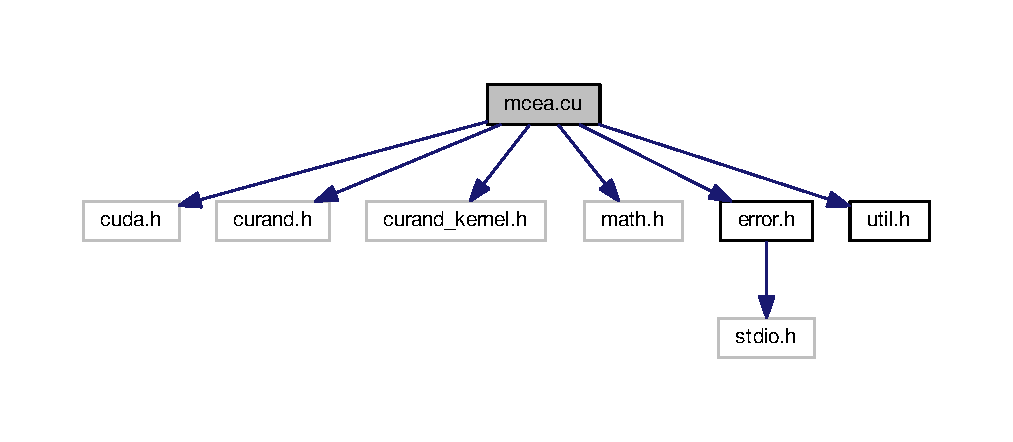
\includegraphics[width=244pt]{mcea_8cu__incl}
\end{center}
\end{figure}
\subsection*{Macros}
\begin{DoxyCompactItemize}
\item 
\#define {\bfseries P\+O\+P\+\_\+\+W\+I\+D\+TH}~10\hypertarget{mcea_8cu_a078505a45e5598fe76de40d43e70e48a}{}\label{mcea_8cu_a078505a45e5598fe76de40d43e70e48a}

\item 
\#define {\bfseries P\+O\+P\+\_\+\+S\+I\+ZE}~((P\+O\+P\+\_\+\+W\+I\+D\+TH $\ast$ (P\+O\+P\+\_\+\+W\+I\+D\+TH + 1)) / 2)\hypertarget{mcea_8cu_aea5b3e4c9df97408e95b67cdf3f992fb}{}\label{mcea_8cu_aea5b3e4c9df97408e95b67cdf3f992fb}

\item 
\#define {\bfseries P\+A\+R\+A\+MS}~50\hypertarget{mcea_8cu_ab0b1e59d96396ba9dca2147f9feb44eb}{}\label{mcea_8cu_ab0b1e59d96396ba9dca2147f9feb44eb}

\item 
\#define {\bfseries O\+B\+JS}~3\hypertarget{mcea_8cu_ad15e0f6530352f2b65cb6147c597c61b}{}\label{mcea_8cu_ad15e0f6530352f2b65cb6147c597c61b}

\end{DoxyCompactItemize}
\subsection*{Functions}
\begin{DoxyCompactItemize}
\item 
\+\_\+\+\_\+global\+\_\+\+\_\+ void \hyperlink{mcea_8cu_a168f0a1a186e2d2fd41bef0cc0dd6c61}{mcea} (float $\ast$population, float $\ast$objectives, float $\ast$utopia\+\_\+vec)
\begin{DoxyCompactList}\small\item\em main kernel \end{DoxyCompactList}\item 
int \hyperlink{mcea_8cu_ae66f6b31b5ad750f1fe042a706a4e3d4}{main} ()
\begin{DoxyCompactList}\small\item\em main function \end{DoxyCompactList}\end{DoxyCompactItemize}


\subsection{Detailed Description}
Main algorithm. Does all the memory management and starts the kernels. 

\subsection{Function Documentation}
\index{mcea.\+cu@{mcea.\+cu}!main@{main}}
\index{main@{main}!mcea.\+cu@{mcea.\+cu}}
\subsubsection[{\texorpdfstring{main()}{main()}}]{\setlength{\rightskip}{0pt plus 5cm}int main (
\begin{DoxyParamCaption}
{}
\end{DoxyParamCaption}
)}\hypertarget{mcea_8cu_ae66f6b31b5ad750f1fe042a706a4e3d4}{}\label{mcea_8cu_ae66f6b31b5ad750f1fe042a706a4e3d4}


main function 

Classic main function. It allocates all memory, generates the population, starts the kernel and collects the results. All parameters changes are made via the \#define statements \index{mcea.\+cu@{mcea.\+cu}!mcea@{mcea}}
\index{mcea@{mcea}!mcea.\+cu@{mcea.\+cu}}
\subsubsection[{\texorpdfstring{mcea(float $\ast$population, float $\ast$objectives, float $\ast$utopia\+\_\+vec)}{mcea(float *population, float *objectives, float *utopia_vec)}}]{\setlength{\rightskip}{0pt plus 5cm}\+\_\+\+\_\+global\+\_\+\+\_\+ void mcea (
\begin{DoxyParamCaption}
\item[{float $\ast$}]{population, }
\item[{float $\ast$}]{objectives, }
\item[{float $\ast$}]{utopia\+\_\+vec}
\end{DoxyParamCaption}
)}\hypertarget{mcea_8cu_a168f0a1a186e2d2fd41bef0cc0dd6c61}{}\label{mcea_8cu_a168f0a1a186e2d2fd41bef0cc0dd6c61}


main kernel 

This kernel runs the whole algorithm. All data structures have to be set up for this. T\+O\+DO\+: implement algorithm 
\begin{DoxyParams}{Parameters}
{\em population} & an array containing all parameters of the whole population. \\
\hline
{\em objectives} & an array containing all objective values (there will be written some new ones) \\
\hline
{\em utopia\+\_\+vec} & a vector containing the best values for each single objective \\
\hline
\end{DoxyParams}

\hypertarget{util_8cu}{}\section{util.\+cu File Reference}
\label{util_8cu}\index{util.\+cu@{util.\+cu}}
{\ttfamily \#include $<$stdlib.\+h$>$}\\*
{\ttfamily \#include $<$stdio.\+h$>$}\\*
{\ttfamily \#include $<$time.\+h$>$}\\*
Include dependency graph for util.\+cu\+:\nopagebreak
\begin{figure}[H]
\begin{center}
\leavevmode
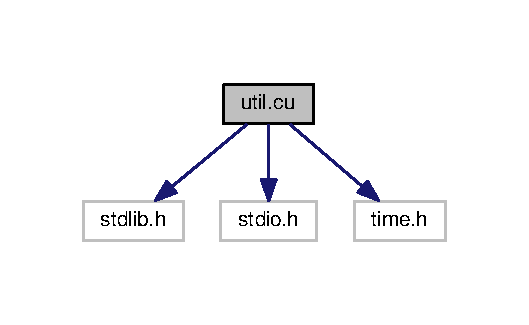
\includegraphics[width=254pt]{util_8cu__incl}
\end{center}
\end{figure}
\subsection*{Functions}
\begin{DoxyCompactItemize}
\item 
float \hyperlink{util_8cu_a6861f8cdbc87ca6342c829824e9084e3}{random\+Float} ()
\item 
void \hyperlink{util_8cu_a1154c3b7555583eb6a784d26f4cb4fcd}{print\+Vector} (float $\ast$vec, int size)
\end{DoxyCompactItemize}


\subsection{Detailed Description}
Utilities. Mostly to display results and generate data. 

\subsection{Function Documentation}
\index{util.\+cu@{util.\+cu}!print\+Vector@{print\+Vector}}
\index{print\+Vector@{print\+Vector}!util.\+cu@{util.\+cu}}
\subsubsection[{\texorpdfstring{print\+Vector(float $\ast$vec, int size)}{printVector(float *vec, int size)}}]{\setlength{\rightskip}{0pt plus 5cm}void print\+Vector (
\begin{DoxyParamCaption}
\item[{float $\ast$}]{vec, }
\item[{int}]{size}
\end{DoxyParamCaption}
)}\hypertarget{util_8cu_a1154c3b7555583eb6a784d26f4cb4fcd}{}\label{util_8cu_a1154c3b7555583eb6a784d26f4cb4fcd}
Prints out a float vector of specifies length to stdout. /param vec pointer to the vector to print out /param size number of elements to print \index{util.\+cu@{util.\+cu}!random\+Float@{random\+Float}}
\index{random\+Float@{random\+Float}!util.\+cu@{util.\+cu}}
\subsubsection[{\texorpdfstring{random\+Float()}{randomFloat()}}]{\setlength{\rightskip}{0pt plus 5cm}float random\+Float (
\begin{DoxyParamCaption}
\item[{void}]{}
\end{DoxyParamCaption}
)}\hypertarget{util_8cu_a6861f8cdbc87ca6342c829824e9084e3}{}\label{util_8cu_a6861f8cdbc87ca6342c829824e9084e3}
Returns a random float number in \mbox{[}0,1). 
%--- End generated contents ---

% Index
\backmatter
\newpage
\phantomsection
\clearemptydoublepage
\addcontentsline{toc}{chapter}{Index}
\printindex

\end{document}
